\documentclass{article}
\usepackage{fontspec}
\setmainfont{Times New Roman}
\usepackage{geometry}
\usepackage{CTEX}
\geometry{papersize={21cm,29.7cm}}
\geometry{left=3.18cm,right=3.18cm,top=2.54cm,bottom=2.54cm}
\usepackage{fancyhdr}
\usepackage{amsmath}
\pagestyle{fancy}
\lhead{学号:202000460020}
\rhead{姓名:苏博南}
\cfoot{\thepage}
\renewcommand{\headrulewidth}{0.4pt}
\renewcommand{\headwidth}{\textwidth}
\usepackage{tikz}
\usetikzlibrary{automata, positioning, arrows}
\usepackage{listings}
\usepackage{float}

\newtheorem{question}{题目}  
\lstset{
	basicstyle=\small\ttfamily,	% 基本样式
		keywordstyle=\color{blue}, % 关键词样式
		commentstyle=\color{gray!50!black!50},   	% 注释样式
		stringstyle=\rmfamily\slshape\color{red}, 	% 字符串样式
	backgroundcolor=\color{gray!0},     % 代码块背景颜色
	frame=leftline,						% 代码框形状
	framerule=12pt,%
		rulecolor=\color{gray!0},      % 代码框颜色
	numbers=left,				% 左侧显示行号往左靠, 还可以为right ,或none,即不加行号
		numberstyle=\footnotesize\itshape,	% 行号的样式
		firstnumber=1,
		stepnumber=1,                  	% 若设置为2,则显示行号为1,3,5
		numbersep=7pt,               	% 行号与代码之间的间距
	aboveskip=.25em, 			% 代码块边框
	showspaces=false,               	% 显示添加特定下划线的空格
	showstringspaces=false,         	% 不显示代码字符串中间的空格标记
	keepspaces=true, 					
	showtabs=false,                 	% 在字符串中显示制表符
	tabsize=2,                     		% 默认缩进2个字符
	captionpos=b,                   	% 将标题位置设置为底部
	flexiblecolumns=true, 			%
	breaklines=true,                	% 设置自动断行
	breakatwhitespace=false,        	% 设置自动中断是否只发生在空格处
	breakautoindent=true,			%
	breakindent=1em, 			%
	title=\lstname,				%
	escapeinside=``,  			% 在``里显示中文
	xleftmargin=1em,  xrightmargin=1em,     % 设定listing左右的空白
	aboveskip=1ex, belowskip=1ex,
	framextopmargin=1pt, framexbottommargin=1pt,
        abovecaptionskip=-2pt,belowcaptionskip=3pt,
	% 设定中文冲突,断行,列模式,数学环境输入,listing数字的样式
	extendedchars=false, columns=flexible, mathescape=true,
	texcl=true,
	fontadjust
}%

\begin{document}

\begin{center}
    \huge{机器学习课程实验七}\\
    \large{\today \quad 苏博南\quad 202000460020}
\end{center}

考虑这样一个数据集,输入为:
\begin{itemize}
	\item [1.] Pregnancies:怀孕次数
	\item [2.] Glucose:口服葡萄糖耐量试验中2小时的血糖浓度
	\item [3.] BloodPressure:舒张压(毫米汞柱)
	\item [4.] SkinThickness:三头肌皮褶厚度(毫米)
	\item [5.] Insulin:2小时血清胰岛素(mu U/ml)
	\item [6.] BMI:体质指数(体重kg/(身高m)\^{}2)
	\item [7.] DiabetesPedigreeFunction:糖尿病谱系功能
	\item [8.] Age:年龄 
\end{itemize} 
输出为一个二分类01,即有无患病。
首先引入必要的库:
\begin{figure}[H]
	\centering
	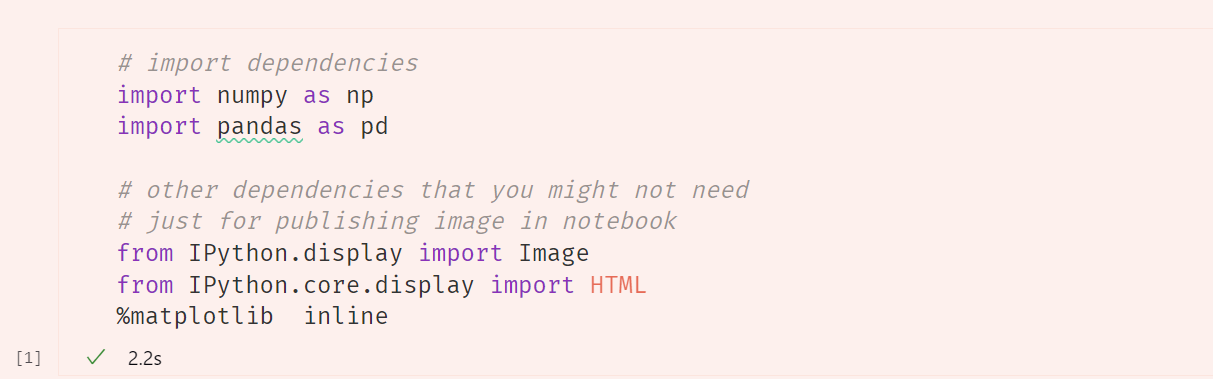
\includegraphics[width=\linewidth]{1.png}
\end{figure}

然后读入数据集:
\begin{figure}[H]
	\centering
	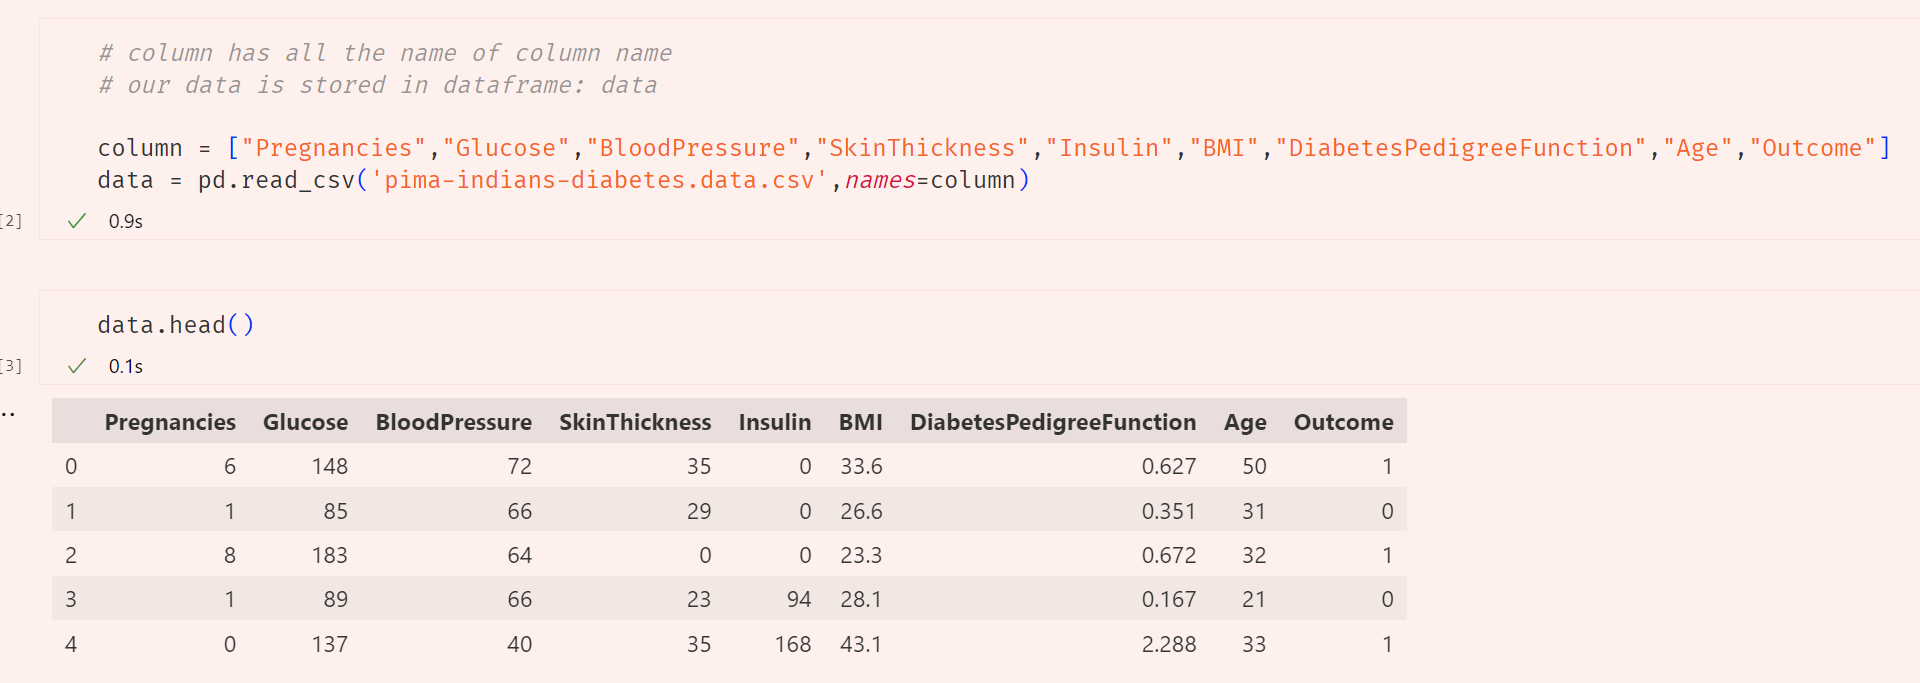
\includegraphics[width=\linewidth]{2.png}
\end{figure}

根据概率学公式:
$$
P(c\;|\;x)=\frac{P(x\;|\;c)P(c)}{P(x)}
$$

其中,\begin{itemize}
	\item [1.] $P(c\;|\;x)$被称为给定特征$x$后,类别$c$的\textbf{后验概率}。
	\item [2.] $P(c)$是类别$c$的\textbf{先验概率}。
	\item [3.] $P(x\;|\;c)$被称为给定类别$c$后特征$x$的\textbf{似然度}。
	\item [4.] $P(x)$被称为特征$x$的\textbf{边缘概率},可以理解为特征的先验主观概率。
\end{itemize}

根据贝叶斯公式,我们分别计算给定特征数据后,outcome0和outcome1的后验概率:
\begin{figure}[H]
	\centering
	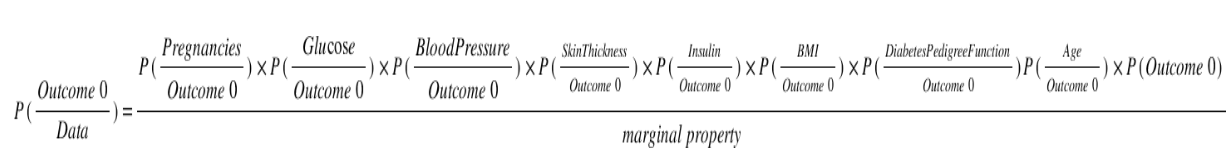
\includegraphics[width=\linewidth]{outcome0.PNG}
\end{figure}
\begin{figure}[H]
	\centering
	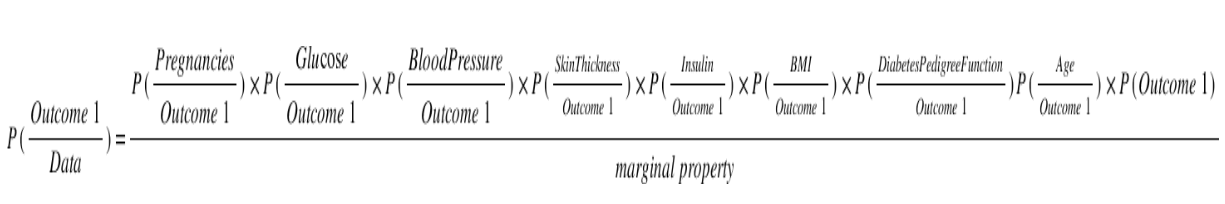
\includegraphics[width=\linewidth]{outcome1.PNG}
\end{figure}

整个朴素贝叶斯分类器就需要五个步骤:
\begin{itemize}
	\item [1.] 计算先验概率。
	\item [2.] 计算似然度。
	\item [3.] 计算边缘概率。
	\item [4.] 利用概率公式计算数据点的后验概率。
	\item [5.] 进行分析。
\end{itemize}
\section{先验概率的计算}
在分类中,我们就把两个类别的先验概率看作是两个类别的样本数量占总样本数的比例:
\begin{figure}[H]
	\centering
	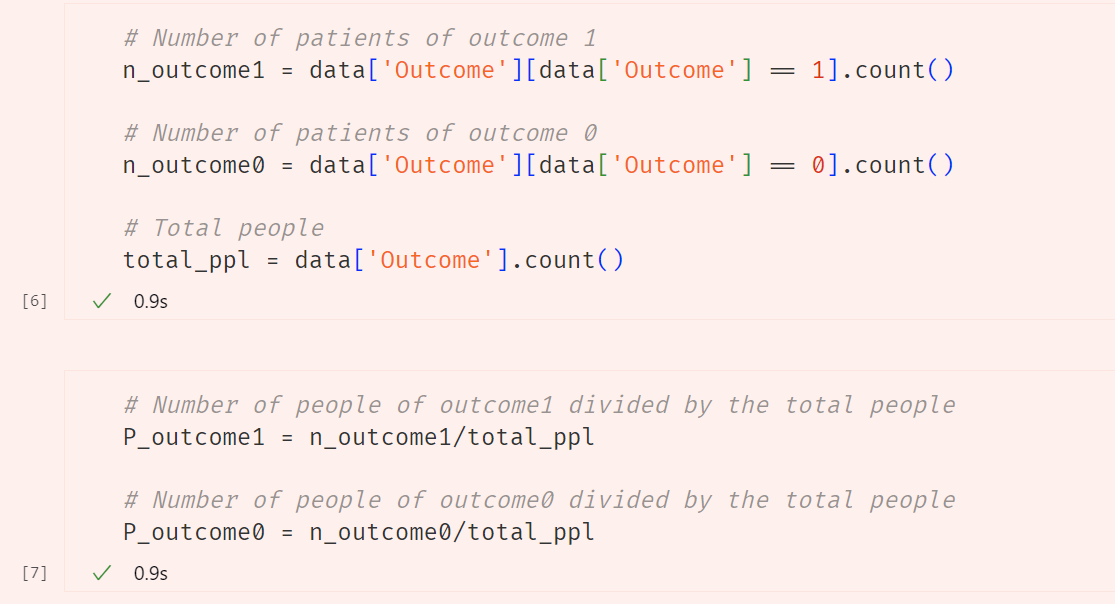
\includegraphics[width=0.7\linewidth]{3.png}
\end{figure}

\section{计算似然度}
$\bullet$ 我们假定给定类别后,每个特征数据都是服从标准正态分布的。

$\bullet$ 根据样本数据,我们可以给出特征分布的参数的无偏估计。以怀孕次数为例:
\begin{figure}[H]
	\centering
	
\includegraphics[width=\linewidth]{bay1.png}
\end{figure}

根据概率学知识,样本均值就是概率分布期望的似然估计,样本方差就是概率分布方差的似然估计。
可以计算得出样本的均值和方差为:
\begin{figure}[H]
	\centering
	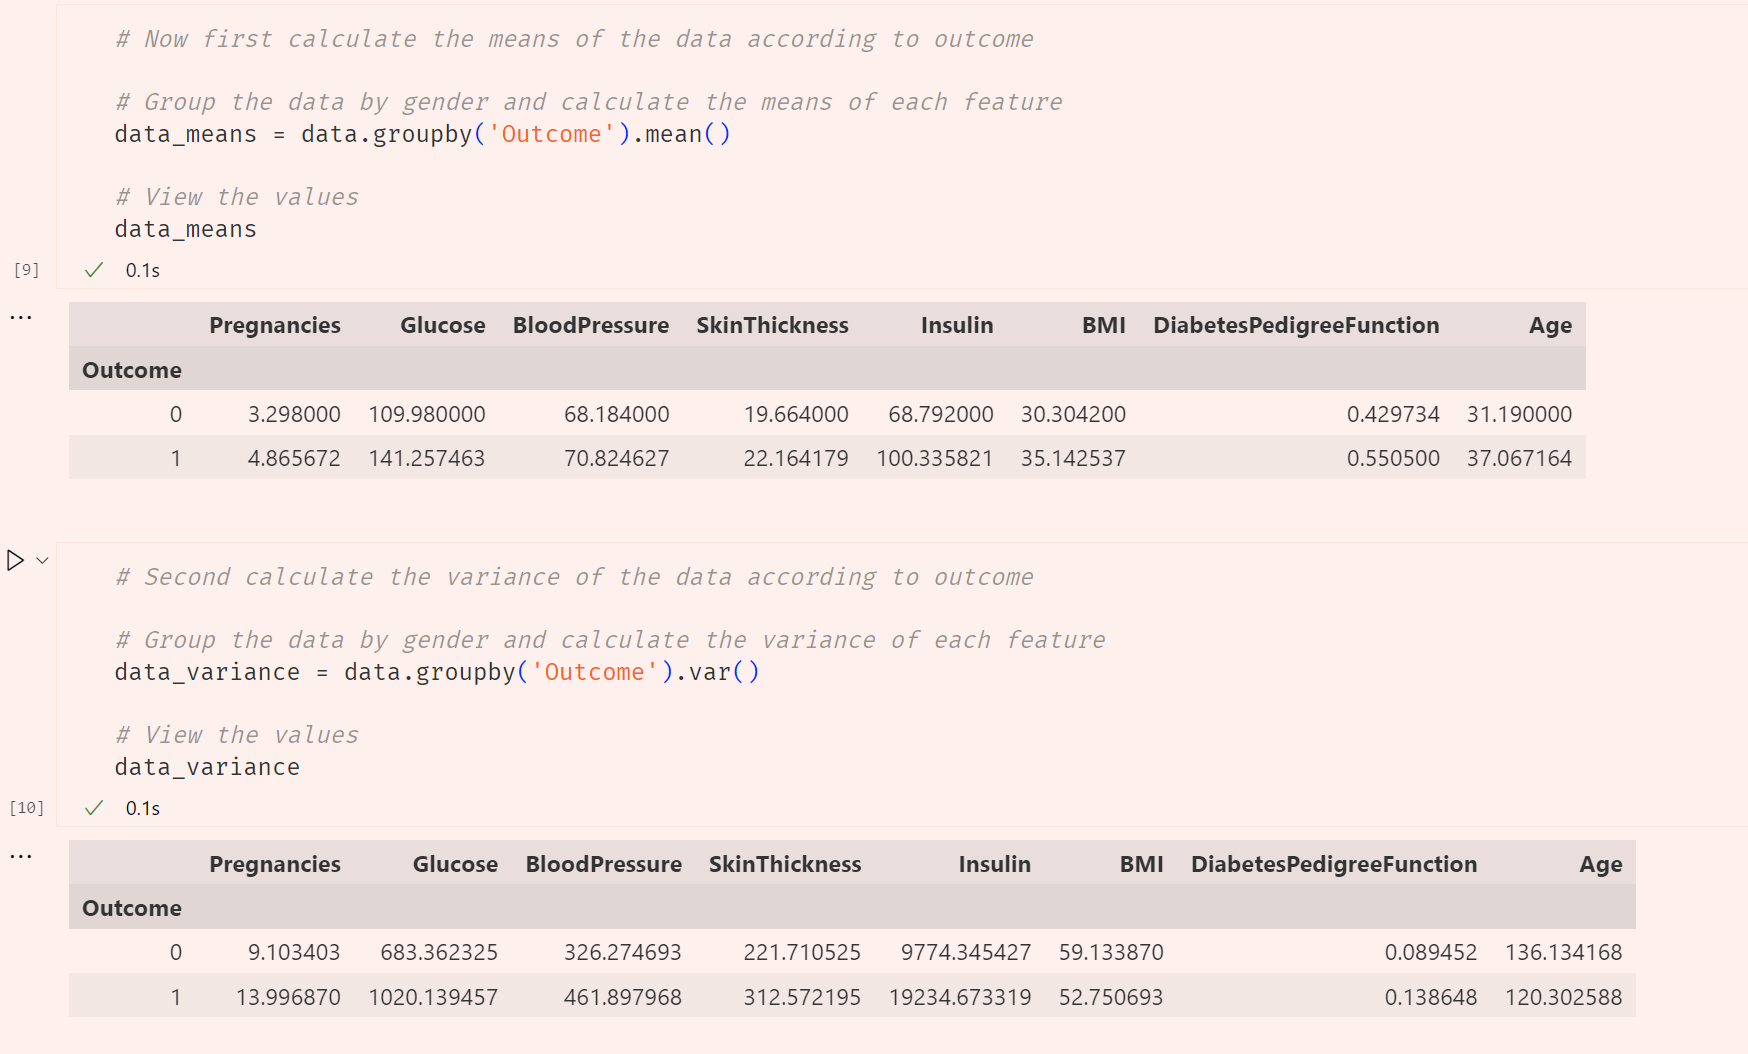
\includegraphics[width=\linewidth]{4.png}
\end{figure}

同理可以计算得到其他特征的概率分布函数。

\section{边缘概率}
现实中边缘概率是极难计算的,我们无法得知每个特征在全体中的占比,就像我们很难知道
"红心的西瓜占全体西瓜的多少"一样。但在朴素贝叶斯分类器中,我们直接
认为边缘概率就是具有特征$x$占全部样本数量的比例。
\section{贝叶斯分类器的应用}
我们用已知的贝叶斯分类器数据去预测新的数据点,计算得到给定data后outcome0和outcome1的数据
比较哪个大确认结果是0还是1。最后在测试集上预测准确率有73\%:
\begin{figure}[H]
	\centering
	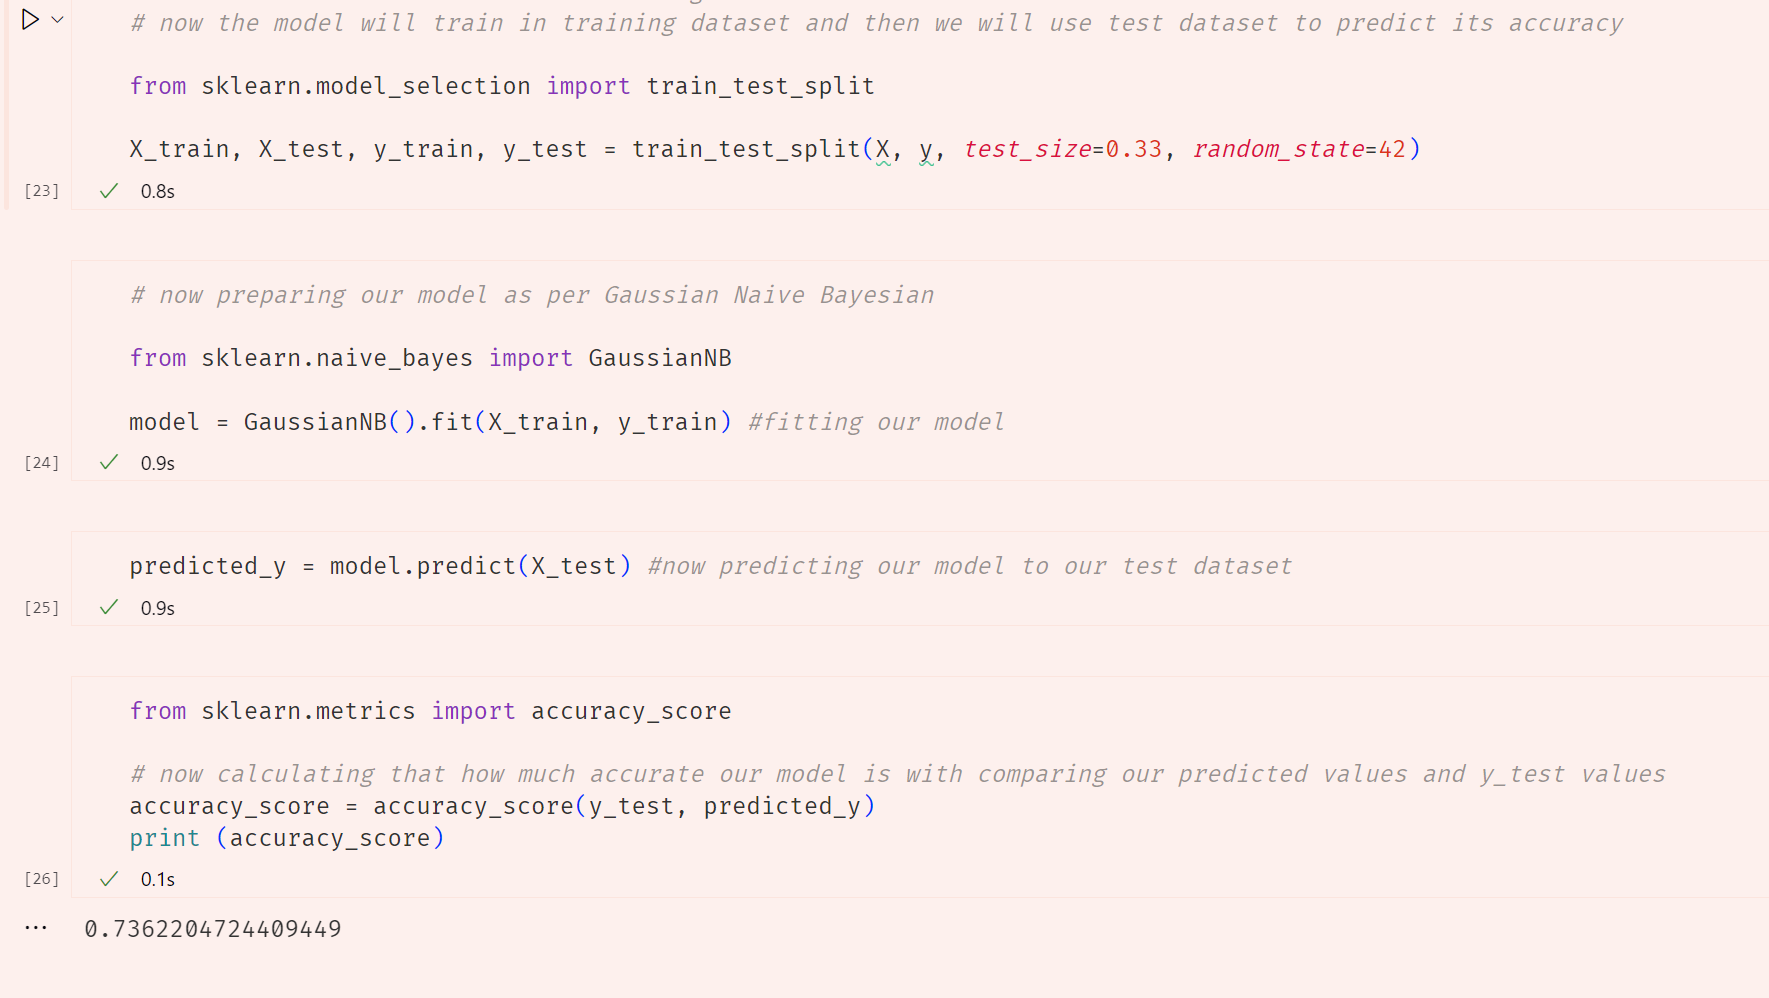
\includegraphics[width=\linewidth]{5.png}
\end{figure}

\end{document}